\documentclass[landscape,letterpaper]{article}
\usepackage[left=5pt,top=5pt,right=20pt]{geometry}
\usepackage{tikz}
\begin{document}

\begin{center}
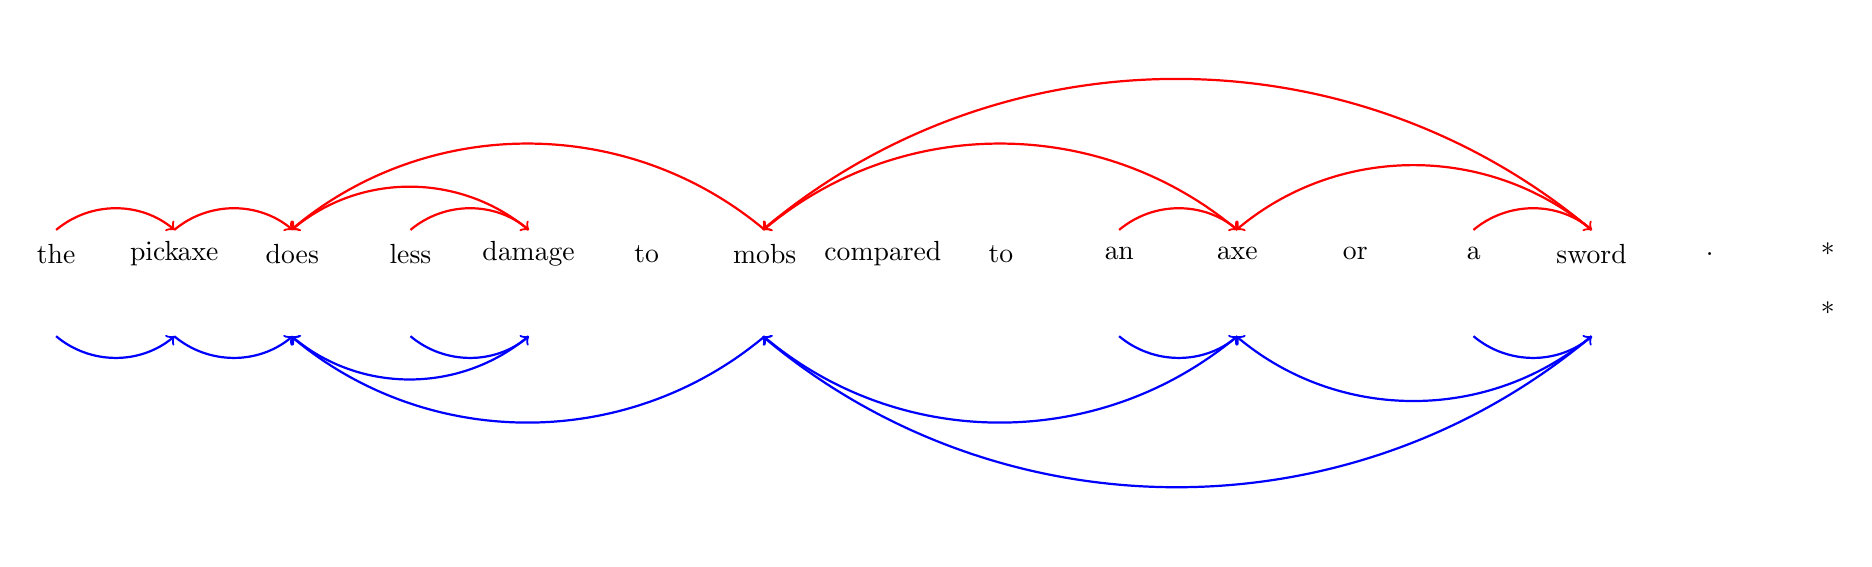
\begin{tikzpicture}[scale=1.5]
\draw(0,0) node {the};
\draw(0,-0.5) node {};
\draw(1,0) node {pickaxe};
\draw(1,-0.5) node {};
\draw(2,0) node {does};
\draw(2,-0.5) node {};
\draw(3,0) node {less};
\draw(3,-0.5) node {};
\draw(4,0) node {damage};
\draw(4,-0.5) node {};
\draw(5,0) node {to};
\draw(5,-0.5) node {};
\draw(6,0) node {mobs};
\draw(6,-0.5) node {};
\draw(7,0) node {compared};
\draw(7,-0.5) node {};
\draw(8,0) node {to};
\draw(8,-0.5) node {};
\draw(9,0) node {an};
\draw(9,-0.5) node {};
\draw(10,0) node {axe};
\draw(10,-0.5) node {};
\draw(11,0) node {or};
\draw(11,-0.5) node {};
\draw(12,0) node {a};
\draw(12,-0.5) node {};
\draw(13,0) node {sword};
\draw(13,-0.5) node {};
\draw(14,0) node {.};
\draw(14,-0.5) node {};
\draw(15,0) node {*};
\draw(15,-0.5) node {*};
\draw[thick,red,->] (0,0.2) arc(130:50:0.78);
\draw[thick,red,->] (1,0.2) arc(130:50:0.78);
\draw[thick,red,->] (3,0.2) arc(130:50:0.78);
\draw[thick,red,->] (4,0.2) arc(50:130:1.56);
\draw[thick,red,->] (6,0.2) arc(50:130:3.12);
\draw[thick,red,->] (9,0.2) arc(130:50:0.78);
\draw[thick,red,->] (10,0.2) arc(50:130:3.12);
\draw[thick,red,->] (12,0.2) arc(130:50:0.78);
\draw[thick,red,->] (13,0.2) arc(50:130:5.46);
\draw[thick,red,->] (13,0.2) arc(50:130:2.34);
\draw[thick,blue,->] (0,-0.7) arc(50:130:-0.78);
\draw[thick,blue,->] (1,-0.7) arc(50:130:-0.78);
\draw[thick,blue,->] (3,-0.7) arc(50:130:-0.78);
\draw[thick,blue,->] (4,-0.7) arc(130:50:-1.56);
\draw[thick,blue,->] (6,-0.7) arc(130:50:-3.12);
\draw[thick,blue,->] (9,-0.7) arc(50:130:-0.78);
\draw[thick,blue,->] (10,-0.7) arc(130:50:-3.12);
\draw[thick,blue,->] (12,-0.7) arc(50:130:-0.78);
\draw[thick,blue,->] (13,-0.7) arc(130:50:-5.46);
\draw[thick,blue,->] (13,-0.7) arc(130:50:-2.34);
\end{tikzpicture}
\end{center}

\end{document}